\section{Gestione dei processi}
Un processo è un programma in esecuzione, è la sequenza di eventi generati dall' elaboratore durante l'esecuzione del programma.
E' una \emph{unità di esecuzione} all'interno di un SO multiprogrammato, composta da risorse fisiche e logiche a lui associate: processore, file aperti, memoria associata, ecc.

Dato un programma posso avere più processi, distinti, che eseguono quel programma. Oguno di essi è una \emph{istanza} diversa dello stesso programma.
Un processo è rappresentabile attraverso:
\begin{itemize}
    \item il codice del programma
    \item i dati sui quali il programma lavora
    \item program counter
    \item valore dei registri
    \item stato dello stack
\end{itemize}
Un processo può avere associate delle risorse:
\begin{itemize}
    \item memoria associata
    \item file aperti
    \item dispositivi I/O associati
\end{itemize}
La memoria di un processo ha spesso questo layout:
\begin{figure}[H]
    \centering
    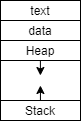
\includegraphics[]{images/3_Gestione_dei_processi/memory_layout.png}
\end{figure}

\subsection{Stati di un processo}
In un sistema operativo monoprogrammato il processo può trovarsi in due stati:
\begin{figure}[H]
    \centering
    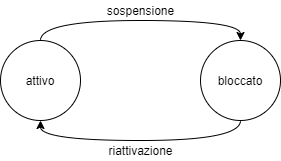
\includegraphics[width=200px]{images/3_Gestione_dei_processi/stati_processo_monoprogrammato.png}
\end{figure}
mentre il processo è attivo sta usando la CPU ed è tutta per lui, quando esegue operazioni sulle periferiche finisce in bloccato perché deve aspettare che la periferica finisca o in genere è in bloccato quando è in attesa di un qualche evento che lo risvegli, quindi non ha la CPU.

In un sistema multiprogrammato se ho più processi che processori lo stato di attivo si divide in due:
\begin{figure}[H]
    \centering
    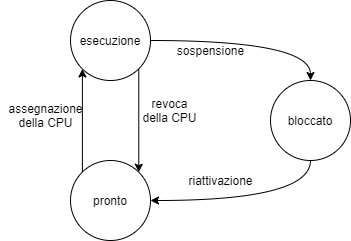
\includegraphics[width=250px]{images/3_Gestione_dei_processi/stati_processo_multiprogrammato.png}
\end{figure}
i processi sono pronti ma sono in attesa che gli venga assegnata la CPU, se eseguo una transazione sull' I/O ritorno in bloccato, posso anche tornare direttamente in pronto a causa della \emph{preemption}.

Lo stato pronto è solitamente una coda di processi, spesso anche lo stato bloccato lo è, sono un insieme di code ognuna delle quali rappresenta una motivazione di blocco.

In definitiva aggiungiamo altri 2 stati:
\begin{figure}[H]
    \centering
    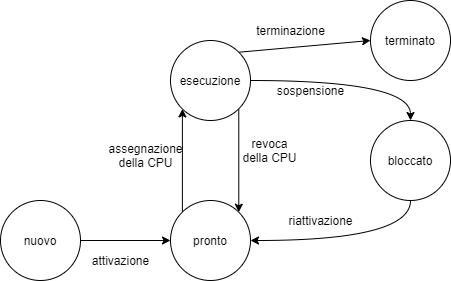
\includegraphics[width=250px]{images/3_Gestione_dei_processi/stati_processo_completo.png}
\end{figure}
si aggiungono lo stato nuovo in cui i processi si trovano all'apertura di un programma, ovvero quando il sistema operativo sta eseguendo il caricamento, e lo stato terminato in cui si va quando il processo giunge al termine e lo fa sapere al sistema operativo.

\subsection{Descrittore di processo}
Un descrittore di processo (Process Control Block, PCB) è una struttura dati gestita dal sistema operativo che modella un processo. Deve contenere, almeno:
\begin{itemize}
    \item nome del processo: un identificatore univoco (es: PID)
    \item stato del processo
    \item modalità di servizio dei processi: informazioni utili allo scheduler per compiere il suo lavoro
    \item informazioni sulla gestione della memoria (es: registro CR3 per la memoria virtuale)
    \item contesto del processo: insieme dei valori dei registri salvato ogni volta che il processo perde l'uso della CPU
    \item utilizzo delle risorse: file aperti, periferiche in uso
    \item identificatore del processo successivo: usato per costruire la coda vera e propria
\end{itemize}

Questi descrittori si trovano tutti in una \emph{tabella dei processi}, è una struttura gestita dal SO che si trova all'interno della memoria di sistema.

I singoli processi poi si trovano sempre in una qualche coda di attesa, su una risorsa o nella coda ready:
\begin{figure}[H]
    \centering
    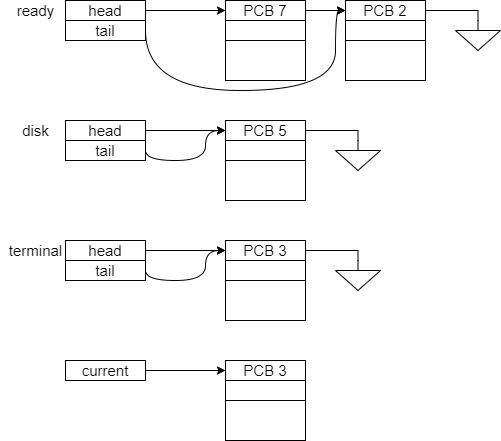
\includegraphics[width=300px]{images/3_Gestione_dei_processi/code_PCB.png}
\end{figure}
in fine c'è sempre un processo correntemente in esecuzione puntato dalla corrispondente variabile.

\subsection{Cambio di contesto}
Il cambio di contesto è un meccanismo utilizzato per cambiare il processo correntemente in esecuzione.
Ciò che deve fare questo meccanismo è:
\begin{itemize}
    \item salvare il contesto del processo in esecuzione nel suo descrittore 
    \item inserire il descrittore del processo salvato in una qualche coda
    \item chiamare lo scheduler per ottenere il nuovo processo da mettere in esecuzione (short term scheduling)
    \item caricare il contesto del processo scelto e metterlo quindi in esecuzione
\end{itemize}
è una componente molto ottimizzata e quindi solitamente scritta in linguaggio macchina.
Fa parte dell' overhead necessario ad ottenere la multiprogrammazione.

Il cambio di contesto potrebbe portare a grossi trasferimenti da e verso la memoria secondaria per allocare e deallocare la memoria del processo; inoltre essendoci la cache di mezzo quando si cambia il contesto essa va svuotata, perciò all' inizio dell' esecuzione si ha un rallentamento dovuto al riempimento della cache.

Alcune architetture di processori mettono a disposizione delle strutture hardware per ottimizzare ancora di più il cambio di contesto.
Questo è ottenuto implementando in hardware più registri ed i descrittori di processo.
Una implementazione, la \emph{SVC - SuperVisor Call} è utilizzata per alcune system call: quando viene lanciata questa istruzione si genera una interruzione interna, cambia solamente il program counter ma lascia i registri così come sono, abbiamo dunque molto meno overhead.

\subsection{Gerarchia dei processi}
Ogni processo è figlio di un altro processo, questo perché solo un processo può richiedere la creazione di altri. Questa gerarchia è tenuta in memoria sempre attraverso informazioni all' interno del descrittore di processo.
Inoltre un processo padre può tracciare lo svolgimento del processo figlio ed all' uscita di un padre tutti i figli vengono terminati.

\subsection{Concorrenza e parallelismo}
Una prima definizione di \emph{concorrenza} potrebbe essere: due o più processi si dicono concorrenti se le loro esecuzioni si sovrappongono nel tempo, questa definizione tuttavia non è sempre accurata, nei sistemi monoprocessore o eseguo il task A o eseguo il task B, quindi non c'è fisicamente una sovrapposizione!
Inoltre questa simultaneità non serve nemmeno in quanto i processi hanno spesso dei tempi morti passati in attesa, quindi aggiungere unità di calcolo spesso è solo uno spreco.
Una definizione più corretta è pertanto: due processi si dicono concorrenti se la prima operazione di uno comincia prima che termini l' ultima dell'altro.

Quello che si usa nei sistemi monoprocessore è quindi un \emph{interleaving}:
\begin{figure}[H]
    \centering
    
\includegraphics[width=300px]{images/3_Gestione_dei_processi/interleaving.png}
\end{figure}
Entrambi i casi sono concorrenti usando la seconda definizione

\subsubsection{Dipendenza tra processi}
Distinguiamo tra due tipi di processi:
\begin{itemize}
    \item indipendenti: due processi sono indipendenti se nessuno dei due influenza l' esecuzione dell' altro.
    Si ha quindi la \emph{proprietà della riproducibilità} cioè: se eseguo lo stesso processo sugli stessi dati tante volte ho la stessa evoluzione temporale.
    Una vera indipendenza però non è mai raggiungibile nella pratica: possiamo avere processi che non condividono informazioni l' uno con l' altro ma che tuttavia concorrono entrambi per l'utilizzo della CPU e per l' utilizzo delle stesse risorse, questa concorrenza porterà sempre ad una diversa evoluzione temporale!
    La vera riproducibilità potrei averla solo su scheduler deterministici e processi che non scambiano informazioni.
    
    \item interagenti: due processi sono interagenti se l' esecuzione di uno è influenzata dall' esecuzione dell' altro e viceversa
\end{itemize}

\subsubsection{Tipi di interazione}
Scindiamo tra due tipi di interazione:
\begin{itemize}
    \item competizione: due processi vogliono accedere alla stessa risorsa che non può essere utilizzata contemporaneamente.
    Tocca al sistema operativo scegliere chi far andare prima e gestire l'accesso in \emph{mutua esclusione} alla risorsa.
    In questo scenario non importa chi va prima e chi va dopo, l' importante è che non vadano insieme.
    
    \item cooperazione: due processi eseguono una attività comune mediante lo scambio di informazioni.
    In questo caso è importante chi arriva prima, si deve quindi risolvere un problema di \emph{sincronizzazione} per permettere le precedenze tra processi.
    Questo è delegato al programmatore tramite opportuna programmazione!
\end{itemize}
La competizione è anche detta \emph{sincronizzazione indiretta} o \emph{implicita}, la cooperazione è anche detta \emph{sincronizzazione diretta} o \emph{esplicita}.

\subsection{Kernel}
E' il componente del sistema operativo che si occupa di creare l' astrazione di \emph{CPU virtuale} usata dai processi, implementa inoltre le funzioni di risposta alle interruzioni ed alle eccezioni, il cambio di contesto e le primitive offerte dal sistema.

